\documentclass[tikz,border=8pt]{standalone}
% Shared look for every TikZ diagram. Load with \input{../../tools/tikz-style.tex}
\usepackage[T1]{fontenc}
\usepackage{lmodern}
\renewcommand{\sfdefault}{lmr}  % diagrams use the same serif as the text
\usetikzlibrary{arrows.meta, positioning, shapes.geometric, calc, fit, backgrounds}
\definecolor{cblue}{HTML}{4C78A8}
\definecolor{corange}{HTML}{F58518}
\definecolor{cgreen}{HTML}{54A24B}
\definecolor{cred}{HTML}{E45756}
\definecolor{cpurple}{HTML}{B279A2}
\definecolor{cgrey}{HTML}{6B6B6B}
\tikzset{
  every picture/.style={font=\sffamily, line width=1.2pt},
  box/.style={draw=#1, fill=#1!12, rounded corners=4pt, align=center, inner sep=7pt, minimum height=1.1cm},
  box/.default=cgrey,
  arrow/.style={-{Stealth[length=3mm]}, draw=cgrey, line width=1.4pt},
  title/.style={font=\sffamily\bfseries\Large},
  note/.style={font=\sffamily\small, text=cgrey, align=center},
}
\AtBeginDocument{\hyphenpenalty=10000 \exhyphenpenalty=10000}

\begin{document}
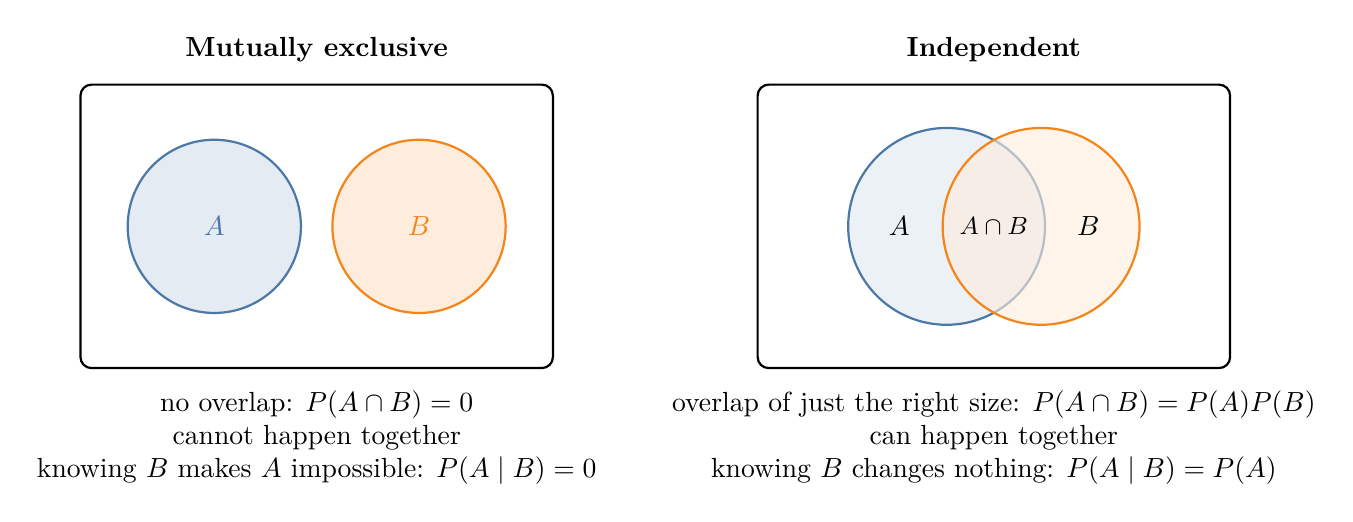
\begin{tikzpicture}
  \begin{scope}
    \draw[thick, rounded corners] (-3,-1.8) rectangle (3,1.8);
    \node[font=\bfseries] at (0,2.25) {Mutually exclusive};
    \draw[thick, cblue, fill=cblue!15] (-1.3,0) circle (1.1) node {$A$};
    \draw[thick, corange, fill=corange!15] (1.3,0) circle (1.1) node {$B$};
    \node[align=center, below] at (0,-1.95) {no overlap: $P(A \cap B) = 0$\\ cannot happen together\\ knowing $B$ makes $A$ impossible: $P(A \mid B) = 0$};
  \end{scope}
  \begin{scope}[xshift=8.6cm]
    \draw[thick, rounded corners] (-3,-1.8) rectangle (3,1.8);
    \node[font=\bfseries] at (0,2.25) {Independent};
    \draw[thick, cblue, fill=cblue!15, fill opacity=0.7] (-0.6,0) circle (1.25);
    \draw[thick, corange, fill=corange!15, fill opacity=0.6] (0.6,0) circle (1.25);
    \node at (-1.2,0) {$A$}; \node at (1.2,0) {$B$}; \node[font=\small] at (0,0) {$A \cap B$};
    \node[align=center, below] at (0,-1.95) {overlap of just the right size: $P(A \cap B) = P(A)P(B)$\\ can happen together\\ knowing $B$ changes nothing: $P(A \mid B) = P(A)$};
  \end{scope}
\end{tikzpicture}
\end{document}
